%
%===============>>  ГРУППА 8-2 МОДУЛЬ 5  <<=============
%
\setmodule{5}

%BEGIN_FOLD % ====>>_____ Занятие 1 _____<<====
\begin{class}[number=1]
	\begin{listofex}
		\item Диагонали прямоугольника равны \( 8 \) и пересекаются
		под углом в \( 60\degree \).
		Найдите меньшую сторону прямоугольника.
		\item Угол при вершине \( A \) ромба \( ABCD \) равен \( 20\degree \). Точки \( M \) и \( N \) --- основания перпендикуляров, опущенных из вершины \( B \) на стороны \( AD \) и \( CD \).
		Найдите углы треугольника \( BMN \).
		\item Квадрат вписан в равнобедренный прямоугольный
		треугольник, причем одна вершина квадрата расположена на
		гипотенузе, противоположная ей вершина совпадает с вершиной
		прямого угла треугольника, а остальные лежат на катетах.
		Найдите сторону квадрата, если катет треугольника равен \( 12 \).
		\item На сторонах \( AB \) и \( CD \) прямоугольника \( ABCD \)
		взяты точки \( K \) и \( M \) так, что \( AKCM \) является ромбом.
		Диагональ \( AC \) составляет со стороной \( AB \) угол \( 30\degree \). Найдите сторону ромба, если наибольшая сторона прямоугольника \( ABCD \) равна \( 3 \).
		\item Докажите, что концы двух различных диаметров
		окружности являются вершинами прямоугольника.
		\item Через середину диагонали KM прямоугольника
		\( KLMN \) перпендикулярно этой диагонали проведена прямая,
		пересекающая стороны \( KL \) и \( MN \) в точках \( A \) и \( B \)
		соответственно. Известно, что \( AB = BM = 6 \).
		Найдите большую сторону прямоугольника.
		\item Окружность, построенная на стороне \( AD \)
		параллелограмма \( ABCD \) как на диаметре, проходит через вершину \( B \) и
		середину стороны \( BC \). Найдите углы параллелограмма.
		\item Решить уравнение:\quad\( (x-17)^2-7(x-17)+10=0 \)
	\end{listofex}
\end{class}
%END_FOLD

%BEGIN_FOLD % ====>>_____ Занятие 2 _____<<====
\begin{class}[number=2]
	\begin{listofex}
		\item Занятие 2
	\end{listofex}
\end{class}
%END_FOLD

%BEGIN_FOLD % ====>>_____ Занятие 3 _____<<====
\begin{class}[number=3]
	\begin{listofex}
		\item Вершины одного параллелограмма по одной лежат на сторонах другого. Докажите, что их центры совпадают.
		\item У двух параллелограммов совпадает пара противоположных вершин. Докажите, что остальные четыре их вершины образуют новый параллелограмм.
		\item На двух соседних сторонах параллелограмма построили равносторонние треугольники, как показано на рисунке. Докажите, что треугольник \( ABC \) равносторонний.
		\begin{center}
			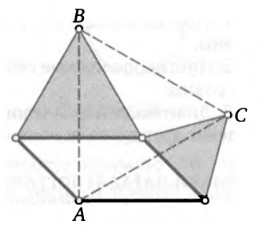
\includegraphics[align=t, width=0.35\linewidth]{\picpath/G82M5H1-1}
		\end{center}
		\item Вершины \( M \) и \( N \) равностороннего треугольника \( BMN \)
		лежат соответственно на сторонах \( AD \) и \( CD \) квадрата \( ABCD \).
		Докажите, что \( MN || AC \).
		\item Через центр квадрата проведены две взаимно
		перпендикулярные прямые. Докажите, что точки пересечения этих
		прямых со сторонами квадрата являются вершинами еще одного
		квадрата.
		\item Через произвольную точку внутри квадрата
		проведены две взаимно перпендикулярные прямые,
		каждая из которых пересекает две противоположные
		стороны квадрата. Докажите, что отрезки этих прямых,
		заключенные внутри квадрата, равны.
	\end{listofex}
\end{class}
%END_FOLD

%BEGIN_FOLD % ====>>_____ Занятие 4 _____<<====
\begin{class}[number=4]
	\begin{listofex}
		\item Занятие 4
	\end{listofex}
\end{class}
%END_FOLD

%BEGIN_FOLD % ====>>_____ Занятие 5 _____<<====
\begin{class}[number=5]
	\begin{listofex}
		\item Занятие 5
	\end{listofex}
\end{class}
%END_FOLD

%BEGIN_FOLD % ====>>_____ Занятие 6 _____<<====
\begin{class}[number=6]
	\begin{listofex}
		\item Занятие 6
	\end{listofex}
\end{class}
%END_FOLD

%BEGIN_FOLD % ====>>_____ Занятие 7 _____<<====
\begin{class}[number=7]
	\begin{listofex}
		\item Занятие 7
	\end{listofex}
\end{class}
%END_FOLD

%BEGIN_FOLD % ====>>_ Домашняя работа 1 _<<====
\begin{homework}[number=1]
	\begin{listofex}
		\item ДЗ 1
	\end{listofex}
\end{homework}
%END_FOLD

%BEGIN_FOLD % ====>>_ Домашняя работа 2 _<<====
\begin{homework}[number=2]
	\begin{listofex}
		\item ДЗ 2
	\end{listofex}
\end{homework}
%END_FOLD

%BEGIN_FOLD % ====>>_ Домашняя работа 3 _<<====
\begin{homework}[number=3]
	\begin{listofex}
		\item ДЗ 3
	\end{listofex}
\end{homework}
%END_FOLD

%BEGIN_FOLD % ====>>_ Проверочная работа _<<====
\begin{exam}
	\begin{listofex}
		\item Проверочная работа
	\end{listofex}
\end{exam}
%END_FOLD
